\documentclass[a4paper,11pt]{article}
\usepackage[utf8]{inputenc}
\usepackage{graphicx}
\usepackage[T2A]{fontenc}
\usepackage[utf8]{inputenc}
\usepackage[english]{babel}
\usepackage{extsizes}
\usepackage{indentfirst}
\usepackage{fancyhdr}
\usepackage{geometry}
\usepackage{amsthm}
\usepackage{amsfonts}
\usepackage{mathtools}
\usepackage{graphicx}
\usepackage{wrapfig}
\usepackage{caption}
\usepackage{amssymb}
\usepackage{booktabs}
\usepackage{dsfont}
\usepackage[toc,page]{appendix}
\usepackage[export]{adjustbox}
\usepackage[percent]{overpic}
\usepackage{pbox}
\usepackage{listings}
\usepackage{xcolor}
\lstset { %
	language=C++,
	backgroundcolor=\color{black!5}, % set backgroundcolor
	basicstyle=\footnotesize,% basic font setting
	keywordstyle=\color[rgb]{0,0,1},
	commentstyle=\color[rgb]{0.026,0.112,0.095},
	stringstyle=\color[rgb]{0.627,0.126,0.941},
	numberstyle=\color[rgb]{0.205, 0.142, 0.73},
	commentstyle=\color{red},
	stringstyle=\color{green}
}

\theoremstyle{plain}
\newtheorem{thm}{Theorem}
\newtheorem{lmm}[thm]{Lemma}
\newtheorem{crlr}[thm]{Corollary}

\theoremstyle{definition}
\newtheorem{defn}[thm]{Definition}
\newtheorem{exmp}[thm]{Example}
\newtheorem{rmrk}[thm]{Remark}
\newtheorem{asmp}[thm]{Assumption}
\newtheorem{prps}[thm]{Proposition}
\newtheorem{cond}[thm]{Conditions}

\graphicspath{{./images/}}

\renewenvironment{proof}{{\scshape Proof:}}{}

\renewcommand{\theenumi}{\roman{enumi}}
\renewcommand{\labelenumi}{(\theenumi)}

\newcommand{\ME}{\mathbb{E}}
\newcommand{\MR}{\mathbb{R}}
\newcommand{\MP}{\mathbb{P}}
\newcommand{\MN}{\mathbb{N}}
\newcommand{\Var}{\mathrm{Var}}
\newcommand{\Cov}{\mathrm{Cov}}
\newcommand{\diag}{\mathrm{diag}}
\newcommand{\tr}{\mathrm{tr}}
\newcommand{\convdistr}{\xrightarrow{\mathcal{L}}}
\newcommand{\convprob}{\xrightarrow{\MP}}
\newcommand{\define}[1]{\textit{\textbf{#1}}}
\bgroup
\def\arraystretch{2}%  1 is the default, change whatever you need
%opening
\title{RandLib documentation}
\author{Aleksandr Samarin}

\begin{document}
	
	\maketitle
	\tableofcontents
	
	\part{General information}
	\section{Calculation of sample moments}
	We use extension of Welford's method from Knuth. For every $n$-th element $x$ we have
	\[
	\begin{aligned}
	\delta &= x - m_1, \\
	m_1' &= m_1 +  \frac{\delta}{n}, \\
	m_2' &= m_2 +  \delta^2 \frac{n-1}{n}, \\
	m_3' &= m_3 + \delta^3 \frac{(n-1)(n-2)}{n^2} - 3\delta \frac{m_2}{n}, \\
	m_4' &= m_4 +  \delta^4 \frac{(n-1)(n^2-3n+3)}{n^3}+6\delta^2 \frac{m_2}{n^2}-4\delta\frac{m_3}{n}.
	\end{aligned}
	\]
	Then $ m_1'$, $\frac{m_2}{n}$, $\mathrm{Skew}(X) = \frac{\sqrt{n}m_3'}{m_2'^{3/2}}$ and $\mathrm{Kurt}(X) = \frac{nm_4'}{m_2'^2}$ (we return excess kurtosis). 
	
	\pagebreak
	\part{Continuous univariate distributions}
	\section{Beta distribution}
		\begin{figure}[!htb]\centering
			\begin{minipage}{0.55\textwidth}
				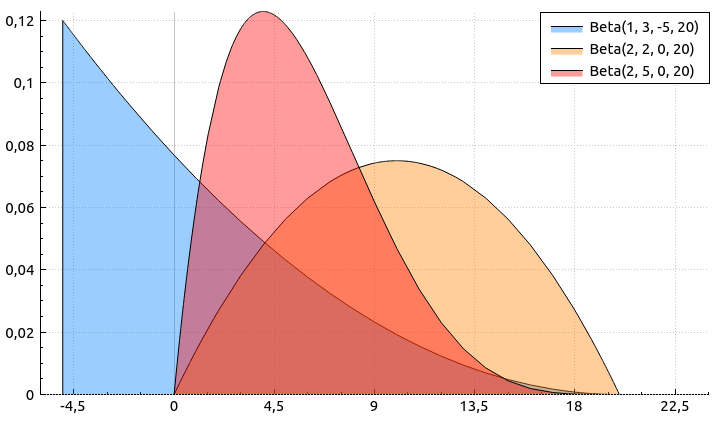
\includegraphics[width=\linewidth, right]{beta_pdf}
				\captionsetup{labelformat=empty}
				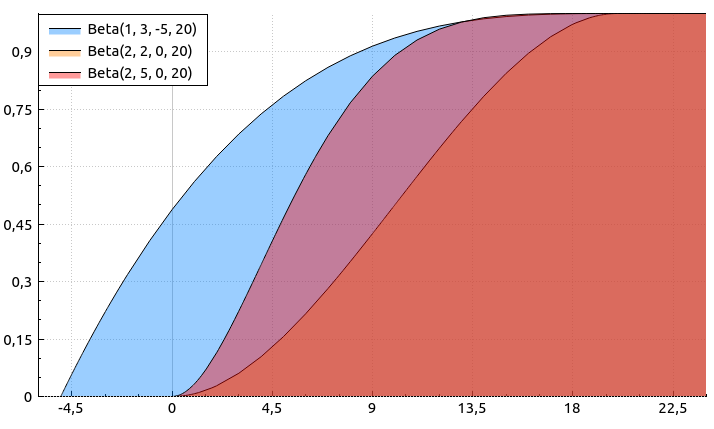
\includegraphics[width=\linewidth, right]{beta_cdf}
				\captionsetup{labelformat=empty}
			\end{minipage}
			\begin{minipage}{0.4\textwidth}
		\begin{tabular}{| r | l |}
			\hline
			Notation & \pbox{\linewidth}{$ X \sim B(\alpha, \beta, a, b)$ \\ $X \sim B(\alpha, \beta)$ with $a=0, b=1$} \\
			\hline
			Parameters & $\alpha, \beta > 0$, $a, b \in \MR$ \\
			\hline
			Support & $x \in [a, b]$  \\
			\hline
			$f(x)$ & $\frac{y^{\alpha - 1}(1 - y)^{\beta - 1}}{(b-a)B(\alpha, \beta)}$ with $y = \frac{x - a}{b - a}$ \\
			\hline
			$F(x)$ & $I_{y}(\alpha, \beta)$ for $y = \frac{x - a}{b - a}$\\
			\hline
			$\ME[X]$ & $a + (b-a)\frac{\alpha}{\alpha + \beta}$ \\
			\hline
			$\Var(X)$ & $(b-a)^2\frac{ \alpha \beta}{(\alpha + \beta)^2 (\alpha + \beta + 1)}$ \\
			\hline
			Median & Searched numerically \\
			\hline
			Mode & $a + (b-a)\frac{\alpha - \beta}{\alpha + \beta - 2}$ for $\alpha, \beta > 1$. \\
			\hline
			$\phi(t)$ & Calculated numerically \\
			\hline
		\end{tabular}
	\end{minipage}
	\end{figure}
	\paragraph{Estimation of shapes with known support.} Assume that $a=0$, $b=1$ and we have a sample $X = (X_1, \dots, X_n)$. Then a log-likelihood function is
	\begin{equation} \label{Beta log-likelihood}
	\begin{aligned}
	\ln \mathcal{L} (\alpha, \beta | X) &= \sum_{i=1}^{n} \ln f(X_i; \alpha, \beta) \\
	& = (\alpha - 1) \sum_{i=1}^{n} \ln X_i + (\beta - 1) \sum_{i=1}^{n}\ln (1-X_i) - n \ln B(\alpha, \beta).
	\end{aligned}  
	\end{equation}
	Differentiating with respect to the shapes, we obtain
	\[
	\frac{\partial \ln \mathcal{L}(\alpha, \beta | X)}{\partial \alpha} = \sum_{i=1}^{n} \ln X_i + n(\psi(\alpha + \beta) - \psi(\alpha)),
	 \]
	\[
	\frac{\partial \ln \mathcal{L}(\alpha, \beta | X)}{\partial \beta} = \sum_{i=1}^{n} \ln (1-X_i) + n(\psi(\alpha + \beta) - \psi(\beta)).
	\]
	Differentiating again we get the Hessian matrix:
	\[
	\mathrm{H}(\ln\mathcal{L}(\alpha,\beta|X)) = n \cdot \begin{pmatrix}
	\psi_1(\alpha+\beta)-\psi_1(\alpha) & \psi_1(\alpha+\beta) \\
	\psi_1(\alpha+\beta) & \psi_1(\alpha+\beta)-\psi_1(\beta)
	\end{pmatrix}.
	\]
	Then we can find the estimators numerically, using Newton's procedure. The initial values of estimators are found via method of moments:
	\[
	\hat{\alpha}_0 = \overline{X}_n \Bigg( \frac{\overline{X}_n(1-\overline{X}_n)}{\hat{s}_n^2} - 1 \Bigg),
	\]
	\[
	\hat{\beta}_0 = (1-\overline{X}_n) \Bigg( \frac{\overline{X}_n(1-\overline{X}_n)}{\hat{s}_n^2} - 1 \Bigg).
	\]
	These values are applicable only if $\hat{s}_n^2 < \overline{X}_n(1-\overline{X}_n)$. If this condition is not satisfied, we set $\hat{\alpha}_0 = \hat{\beta}_0 = 0.001$.\\
	In the general case, when $a \neq 0$ or $b \neq 1$, we use the following transformation:
	\[ Y_i = \frac{X_i - a}{b - a} \]
	and estimate parameters, using sample $Y$.
	
	\subsection{Arcsine distribution}
	Relation to Beta distribution: \[ X \sim B(1-\alpha, \alpha, a, b). \]
	\paragraph{Estimation of shape.} For Arcsine distribution log-likelihood function \eqref{Beta log-likelihood} turns into
	\[
	\ln \mathcal{L} (\alpha | X) = -\alpha \sum_{i=1}^{n} \ln X_i + (\alpha - 1) \sum_{i=1}^{n}\ln (1-X_i) - n \ln B(1-\alpha, \alpha).
	\]
	Taking the derivative with respect to $\alpha$ we get
	\[ 
	\frac{\partial \ln\mathcal{L}(\alpha | X)}{\partial \alpha} = \sum_{i=1}^{n} \ln \frac{1-X_i}{X_i} + n\pi \cot(\pi \alpha).
	\]
	Therefore, maximum-likelihood function is
	\[ \hat{\alpha} = -\frac{1}{\pi} \mathrm{atan}\Bigg(\frac{n\pi}{\sum_{i=1}^{n} \ln \frac{1-X_i}{X_i}}\Bigg). \]
	If $\hat{\alpha}$ is negative, we add $1$, because $\frac{\mathrm{atan}}{\pi} \in (-0.5, 0.5)$, while $\alpha \in (0, 1)$.
	
	\subsection{Balding-Nichols distribution}
	Notation: \[ X \sim \mathrm{Balding-Nichols}(p, F) \] with $p, F \in (0, 1)$.
	Relation to Beta distribution: \[ X \sim B(pF', (1 - p)F') \] with $F' = (1 - F) / F$.
	
	\subsection{Uniform distribution}
	\begin{figure}[!htb]\centering
		\begin{minipage}{0.55\textwidth}
			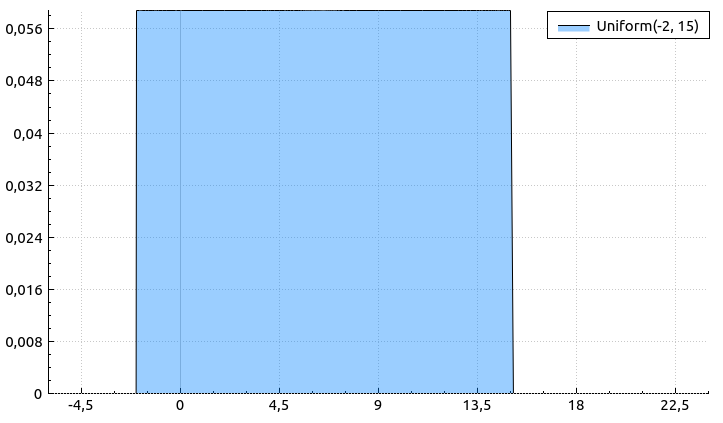
\includegraphics[width=\linewidth, right]{uniform_pdf}
			\captionsetup{labelformat=empty}
			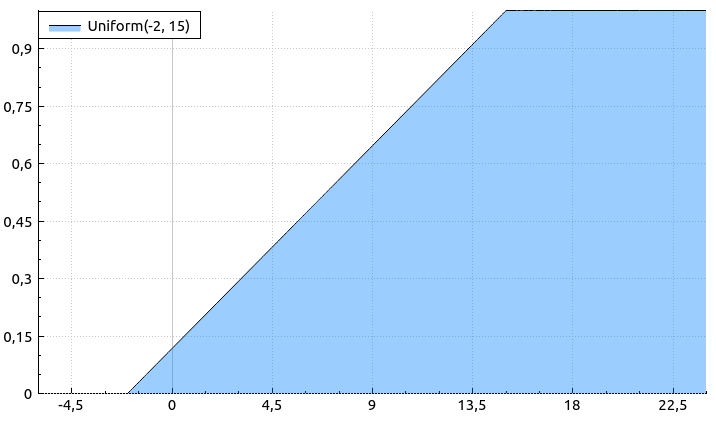
\includegraphics[width=\linewidth, right]{uniform_cdf}
			\captionsetup{labelformat=empty}
		\end{minipage}
		\begin{minipage}{0.4\textwidth}
			\begin{tabular}{| r | l |}
				\hline
				Notation & $ X \sim \mathcal{U}(a, b)$ \\
				\hline
				Parameters & $a, b \in \MR$ \\
				\hline
				Support & $x \in [a, b]$  \\
				\hline
				$f(x)$ & $\frac{1}{b - a}$ \\
				\hline
				$F(x)$ & $\frac{x - a}{b - a}$\\
				\hline
				$\ME[X]$ & $ \frac{a+b}{2}$ \\
				\hline
				$\Var(X)$ & $\frac{(b-a)^2}{12}$ \\
				\hline
				Median & $\frac{a+b}{2}$ \\
				\hline
				Mode & doesn't exist \\
				\hline
				$\phi(t)$ & $ \frac{e^{itb}-e^{ita}}{it(b-a)} $ \\
				\hline
			\end{tabular}
		\end{minipage}
	\end{figure}
	
	Relation to Beta distribution: \[X \sim B(1, 1, a, b). \]
	\paragraph{Estimation of support.}
	\subparagraph{Frequentist inference.} Likelihood function is
	\[
	\mathcal{L}(a, b | X) = \frac{1}{(b-a)^n} \mathbf{1}_{ \{ X_i \in [a, b] \ \forall i = 1, \dots, n \} }.
	\]
	Therefore, $\mathcal{L}(a, b | X)$ is the largest for $\hat{b} = X_{(n)}$ and $\hat{a} = X_{(1)}$. However, using the fact that $X_{(k)} \sim B(k, n+1-k, a, b)$, these are biased estimators:
	\[ \ME[X_{(1)}] = \frac{an + b}{n+1} \quad \text{and} \quad \ME[X_{(n)}] = \frac{a + bn}{n+1}.  \]
	To get unbiased estimators we make the transformations:
	\[ \tilde{a} = \frac{nX_{(1)} - X_{(n)} }{n-1} \quad \text{and} \quad  \tilde{b} = \frac{nX_{(n)} - X_{(1)} }{n-1}. \]
	Then we get
	\[ 
	\ME[\tilde{a}] = \frac{n\ME[X_{(1)}] - \ME[X_{(n)}]}{n-1} = \frac{n(an+b)-(a+bn)}{n^2-1} = a.
	\]
	Analogously, $\ME[\tilde{b}] = b$.
	\subparagraph{Bayesian inference.} Let us say, we try to estimate $\theta = b-a$ with known $a$. We set the prior distribution $\theta \sim \mathrm{Pareto}(\alpha, \sigma)$:
	\[
	h(\theta|\alpha, \sigma) = \frac{\alpha \sigma^\alpha}{\theta^{\alpha + 1}} \mathbf{1}_{\{\theta \geq \sigma\}}.
	\]
	The density of posterior distribution is
	\[
	f(\theta|X) \propto \frac{\alpha \sigma^\alpha}{\theta^{\alpha+n+1}} \mathbf{1}_{\{\theta \geq \max(\sigma, X_{(n)}-a) \}} \sim \mathrm{Pareto}(\alpha + n, \max(\sigma, X_{(n)}-a) ).
	\]
	Hence, Bayesian estimator is
	\[  
	\ME[\theta|X] = \frac{\alpha + n}{\alpha + n - 1}\max(\sigma, X_{(n)}-a)
	\]
	and MAP estimator is
	\[
	\theta_{MAP} = \max(\sigma, X_{(n)}-a).
	\]
	
	\section{Beta-prime distribution}
		\begin{figure}[!htb]\centering
		\begin{minipage}{0.55\textwidth}
			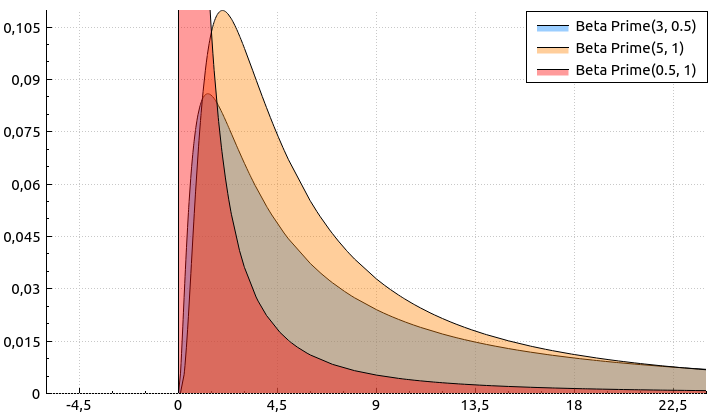
\includegraphics[width=\linewidth, right]{beta_prime_pdf}
			\captionsetup{labelformat=empty}
			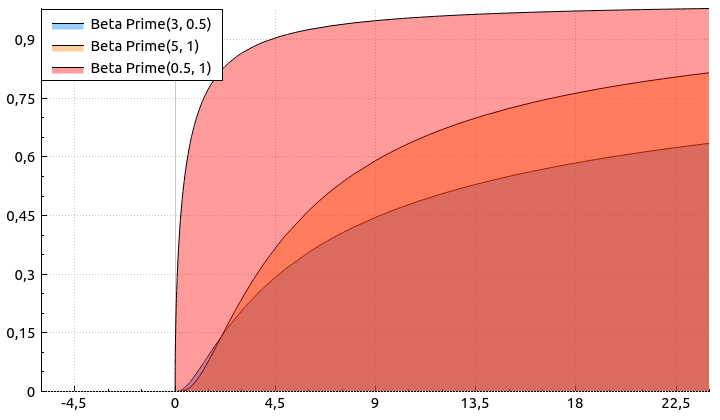
\includegraphics[width=\linewidth, right]{beta_prime_cdf}
			\captionsetup{labelformat=empty}
		\end{minipage}
		\begin{minipage}{0.4\textwidth}
			\begin{tabular}{| r | l |}
				\hline
				Notation & $X \sim B'(\alpha, \beta)$ \\
				\hline
				Parameters & $\alpha, \beta > 0$ \\
				\hline
				Support & $x \in \MR^+$  \\
				\hline
				$f(x)$ & $\frac{x^{\alpha - 1}(1 + x)^{-\alpha - \beta}}{B(\alpha, \beta)}$ \\
				\hline
				$F(x)$ & $I_{\frac{x}{1+x}}(\alpha, \beta)$\\
				\hline
				$\ME[X]$ & $ \frac{\alpha}{\beta - 1}\mathbf{1}_{\{\beta > 1 \} } + \infty \mathbf{1}_{\{\beta \leq 1\} } $ \\
				\hline
				$\Var(X)$ & $\frac{ \alpha (\alpha +\beta - 1) }{ (\beta-2)(\beta-1)^2 }$, if $\beta > 1$ \\
				\hline
				Median & Searched numerically \\
				\hline
				Mode & $\max\big( \frac{\alpha-1}{\beta+1}, 0 \big)$. \\
				\hline
				$\phi(t)$ & Calculated numerically \\
				\hline
			\end{tabular}
		\end{minipage}
	\end{figure}
	Relation to other distributions:
	\[\frac{X}{1+X} \sim B(\alpha, \beta),\]
	\[
	\frac{\beta}{\alpha}X \sim F(2\alpha, 2\beta ).
	\]
	\paragraph{Estimation of shapes.} Using relationship with Beta distribution we transform the sample:
	\[ Y_i = \frac{X_i}{1+X_i}, \quad 1 \leq i \leq N, \]
	and run BetaRand estimation for $Y$.

	
	\section{Exponentially-modified Gaussian distribution}
	\begin{center}
		\begin{tabular}{| r | l |}
			\hline
			Notation & $X \sim \mathrm{EMG}(\mu, \sigma, \lambda)$ \\
			\hline
			Parameters & $\mu \in \MR, \sigma > 0, \lambda > 0$ \\
			\hline
			Support & $x \in \MR$  \\
			\hline
			$f(x)$ & $...  $ \\
			\hline
			$F(x)$ & $... $\\
			\hline
			$\ME[X]$ & $ \mu + 1 / \lambda$ \\
			\hline
			$\Var(X)$ & $\sigma^2 + 1/\lambda^2$ \\
			\hline
			Median & Searched numerically \\
			\hline
			Mode & Searched numerically \\
			\hline
			$\phi(t)$ & $ ... $ \\
			\hline
		\end{tabular}
	\end{center}
	\section{F-distribution}
		\begin{center}
			\begin{tabular}{| r | l |}
				\hline
				Notation & $X \sim \mathrm{F}(d_1, d_2)$ \\
				\hline
				Parameters & $d_1, d_2 > 0$ \\
				\hline
				Support & $x \in \MR^+$  \\
				\hline
				$f(x)$ & $\frac{\sqrt{\frac{(d_1 x)^{d_1} {d_2}^{d_2} }{(d_1x+d_2)^{d_1+d_2}}}}{x B\Big(\frac{d_1}{2},\frac{d_2}{2}\Big)}  $ \\
				\hline
				$F(x)$ & $ I_{\frac{d_1x}{d_1x+d_2}}\Big(\frac{d_1}{2},\frac{d_2}{2}\Big) $\\
				\hline
				$\ME[X]$ & $ \frac{d_2}{d_2-2}$ for $ d_2 > 2 $ \\
				\hline
				$\Var(X)$ & $\frac{2d_2^2(d_1+d_2-2)}{d_1(d_2-2)^2(d_2-4)}$ for $d_2 > 4$ \\
				\hline
				Median & Searched numerically \\
				\hline
				Mode & $\max\Big(\frac{d_2(d_1-2)}{d_1(d_1+2)}, 0\Big)$ \\
				\hline
				$\phi(t)$ & Calculated numerically \\
				\hline
			\end{tabular}
		\end{center}
		Relation to other distributions:
		\[
		\frac{d_1X}{d_2 + d_1X} \sim B\bigg(\frac{d_1}{2}, \frac{d_2}{2} \bigg),
		\]
		\[
		\frac{d_1}{d_2}X \sim B'\bigg(\frac{d_1}{2}, \frac{d_2}{2} \bigg).
		\]
		
		
	\section{Gamma distribution}
	\begin{figure}[!htb]\centering
		\begin{minipage}{0.55\textwidth}
			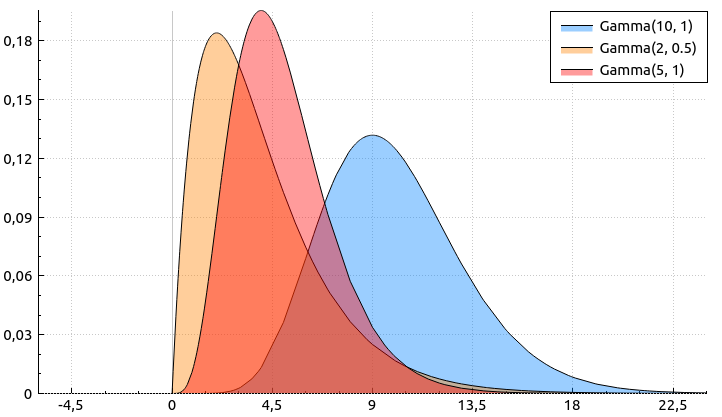
\includegraphics[width=\linewidth, right]{gamma_pdf}
			\captionsetup{labelformat=empty}
			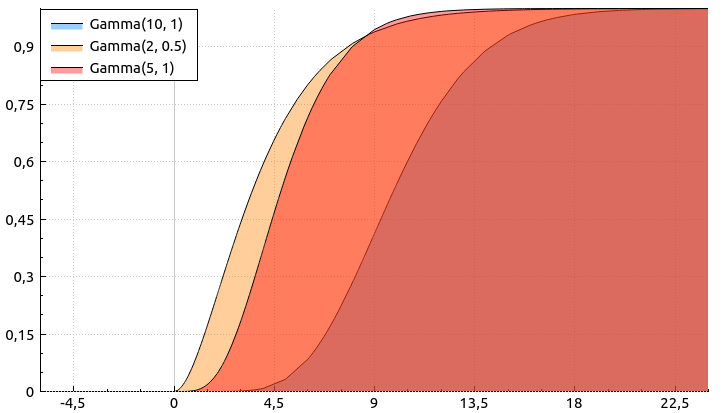
\includegraphics[width=\linewidth, right]{gamma_cdf}
			\captionsetup{labelformat=empty}
		\end{minipage}
		\begin{minipage}{0.4\textwidth}
			\begin{tabular}{| r | l |}
				\hline
				Notation & $X \sim \Gamma(\alpha, \beta)$ \\
				\hline
				Parameters & $\alpha > 0, \beta > 0$ \\
				\hline
				Support & $x \in \MR^+$  \\
				\hline
				$f(x)$ & $\frac{\beta^\alpha}{\Gamma(\alpha)} x^{\alpha-1}e^{-\beta x}  $ \\
				\hline
				$F(x)$ & $P(\alpha, \beta x) $\\
				\hline
				$\ME[X]$ & $ \frac{\alpha}{\beta}$ \\
				\hline
				$\Var(X)$ & $\frac{\alpha}{\beta^2}$ \\
				\hline
				Median & Searched numerically \\
				\hline
				Mode & $\max\big(\frac{\alpha - 1}{\beta}, 0\big)$ \\
				\hline
				$\phi(t)$ & $ \Big( 1-\frac{it}{\beta} \Big)^{-\alpha}$ \\
				\hline
			\end{tabular}
		\end{minipage}
	\end{figure}
	
	\paragraph{Estimation of parameters.}
	\subparagraph{Frequentist inference.} Log-likelihood function:
	\[
	\ln \mathcal{L}(\alpha, \beta|X) =  n \alpha \ln \beta - n \ln \Gamma(\alpha) + (\alpha - 1) \sum_{i=1}^{n} \ln X_i - \beta \sum_{i=1}^{n} X_i.
	\]
	Derivatives:
	\[
	\frac{\partial \ln \mathcal{L}(\alpha, \beta | X) }{\partial \alpha} = n \ln \beta - n \psi (\alpha) + \sum_{i=1}^{n} \ln X_i,
	\]
	\[
	\frac{\partial \ln \mathcal{L}(\alpha, \beta | X) }{\partial \beta} = \frac{n \alpha}{\beta} - \sum_{i=1}^{n} X_i.
	\]
	While the solution for the second equation is analytic:
	\[
	\hat{\beta} = \frac{\alpha}{\overline{X}_n},
	\]
	the first equation is solved numerically, using second derivative:
	\[
	\frac{\partial^2 \ln \mathcal{L}(\alpha, \beta | X) }{\partial \alpha^2} = - n \psi_1 (\alpha),
	\]
	or if $\beta$ is unknown:
	\[
	\frac{\partial^2 \ln \mathcal{L}(\alpha, \beta | X) }{\partial \alpha^2} = - n \psi_1 (\alpha) + \frac{n}{\alpha},
	\]
	Moreover, the maximum-likelihood estimation of rate $\beta$ is biased. Unbiased estimator would be
	\[
	\tilde{\beta} = \frac{\alpha}{\overline{X}_n} \Big(1 - \frac{1}{n}\Big).
	\]
	\subparagraph{Bayesian inference.} We suppose that prior distribution of rate $\beta$ is $\Gamma(\kappa, \theta)$:
	\[
	h(\beta) = \frac{\theta^\kappa}{\Gamma(\kappa)} \beta^{\kappa-1}e^{-\theta \beta}.
	\]
	Then
	\[
	f(\beta | X) \propto \beta^{\alpha n} e^{-\beta \sum_{i=1}^{n} X_i } \cdot \beta^{\kappa-1}e^{-\theta \beta} \sim \operatorname{\Gamma}\Big(\alpha n + \kappa, \theta +\sum_{i=1}^{n} X_i \Big).
	\]
	Therefore, Bayesian estimator is
	\[
	\ME[\beta|X] = \frac{\alpha n + \kappa}{\theta +\sum_{i=1}^{n} X_i},
	\]
	and MAP estimator is
	\[
	\beta_{MAP} = \frac{\alpha n + \kappa - 1}{\theta +\sum_{i=1}^{n} X_i}.
	\]
	
	\subsection{Chi-squared distribution}
	Relation to Gamma distribution:
	\subsection{Erlang distribution}
	The only difference between Gamma and Erlang distributions is that a second one takes an integer shape parameter $k$.
	\subsection{Exponential distribution}
	\begin{figure}[!htb]\centering
		\begin{minipage}{0.55\textwidth}
			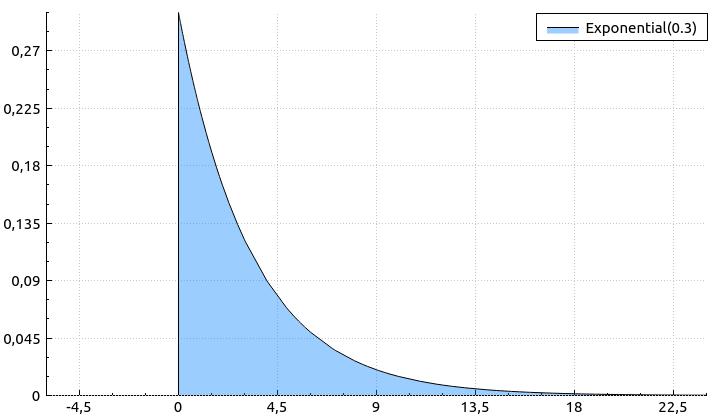
\includegraphics[width=\linewidth, right]{exponential_pdf}
			\captionsetup{labelformat=empty}
			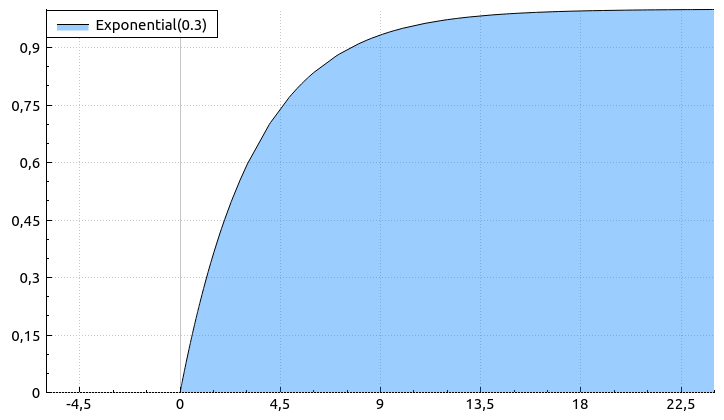
\includegraphics[width=\linewidth, right]{exponential_cdf}
			\captionsetup{labelformat=empty}
		\end{minipage}
		\begin{minipage}{0.4\textwidth}
		\begin{tabular}{| r | l |}
			\hline
			Notation & $X \sim \mathrm{Exp}(\lambda)$ \\
			\hline
			Parameters & $\lambda > 0$ \\
			\hline
			Support & $x \in \MR^+$  \\
			\hline
			$f(x)$ & $\lambda e^{-\lambda x}  $ \\
			\hline
			$F(x)$ & $1-e^{-\lambda x} $\\
			\hline
			$\ME[X]$ & $ \frac{1}{\lambda}$ \\
			\hline
			$\Var(X)$ & $\frac{1}{\lambda^2}$ \\
			\hline
			Median & $\frac{\ln(2)}{\lambda}$ \\
			\hline
			Mode & $0$ \\
			\hline
			$\phi(t)$ & $ \frac{\lambda}{\lambda-it}$ \\
			\hline
		\end{tabular}
		\end{minipage}
	\end{figure}

	Relation to Gamma distribution:
	$X \sim \Gamma(1, \lambda).$
	Hence, estimation of parameter $\lambda$ is the particular case of estimation of rate $\beta$ for Gamma distribution.
	
	
	\section{Geometric Stable distribution}
	\begin{figure}[!htb]\centering
		\begin{minipage}{0.55\textwidth}
			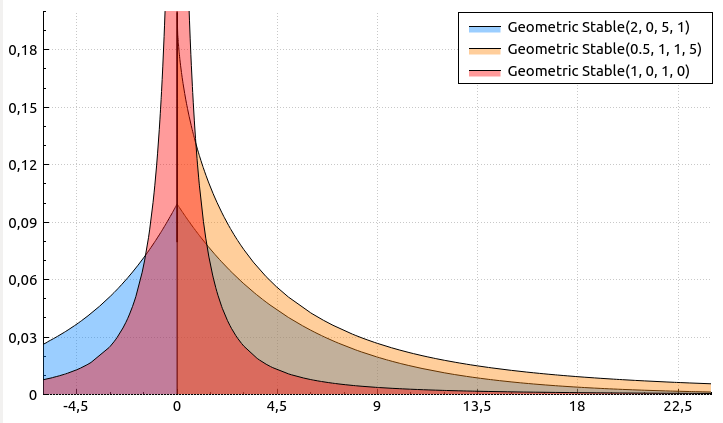
\includegraphics[width=\linewidth, right]{geometric_stable_pdf}
			\captionsetup{labelformat=empty}
			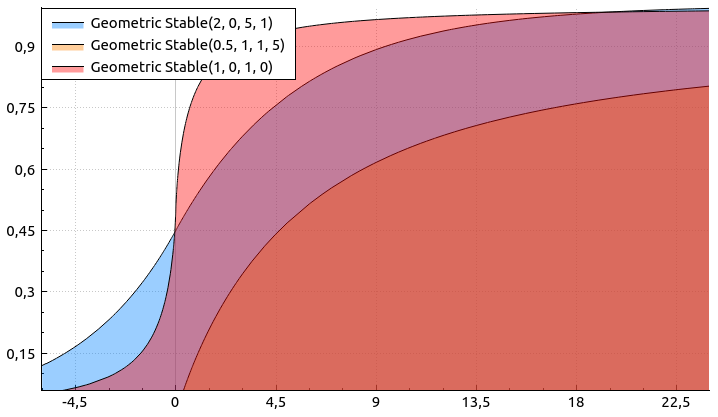
\includegraphics[width=\linewidth, right]{geometric_stable_cdf}
			\captionsetup{labelformat=empty}
		\end{minipage}
		\begin{minipage}{0.4\textwidth}
			\begin{tabular}{| r | l |}
				\hline
				Notation & $X \sim \mathrm{GS}_\alpha(\beta, \gamma, \mu)$ \\
				\hline
				Parameters & \pbox{\linewidth}{$\alpha \in (0, 2], \beta \in [-1, 1],$\\ $\gamma > 0, \mu \in \MR $} \\
				\hline
				Support & $x \in ...$  \\
				\hline
				$f(x)$ & Calculated numerically \\
				\hline
				$F(x)$ & Calculated numerically \\
				\hline
				$\ME[X]$ & $ k + \lambda$ \\
				\hline
				$\Var(X)$ & $2(k+2\lambda)$ \\
				\hline
				Median & Searched numerically \\
				\hline
				Mode & Searched numerically \\
				\hline
				$\phi(t)$ & $ ...$ \\
				\hline
			\end{tabular}
		\end{minipage}
	\end{figure}
	
	\subsection{Asymmetric Laplace distribution}

	\subsection{Laplace distribution}
	
	\section{Noncentral Chi-Squared distribution}
	\begin{figure}[!htb]\centering
	\begin{minipage}{0.55\textwidth}
		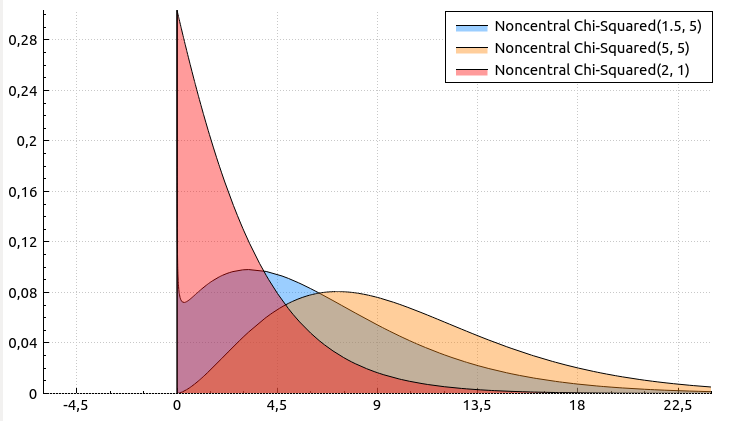
\includegraphics[width=\linewidth, right]{noncentral_chi-squared_pdf}
		\captionsetup{labelformat=empty}
		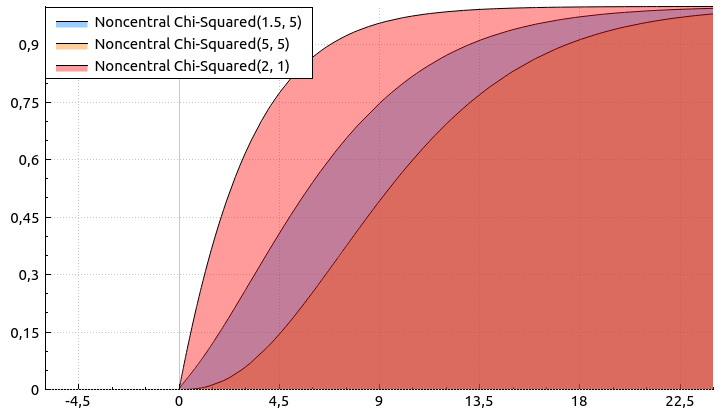
\includegraphics[width=\linewidth, right]{noncentral_chi-squared_cdf}
		\captionsetup{labelformat=empty}
	\end{minipage}
	\begin{minipage}{0.4\textwidth}
		\begin{tabular}{| r | l |}
			\hline
			Notation & $X \sim \chi'^2_k(\lambda)$ \\
			\hline
			Parameters & $k > 0, \lambda > 0$ \\
			\hline
			Support & $x \in \MR^+$  \\
			\hline
			$f(x)$ & $...  $ \\
			\hline
			$F(x)$ & $P_{\frac{k}{2}}(...) $\\
			\hline
			$\ME[X]$ & $ k + \lambda$ \\
			\hline
			$\Var(X)$ & $2(k+2\lambda)$ \\
			\hline
			Median & Searched numerically \\
			\hline
			Mode & Searched numerically \\
			\hline
			$\phi(t)$ & $ \frac{\exp{\frac{it\lambda}{1-2it}}}{(1-2it)^{k/2}}$ \\
			\hline
		\end{tabular}
	\end{minipage}
    \end{figure}
	
	
	\section{Planck distribution}
	
	\begin{figure}[!htb]\centering
		\begin{minipage}{0.55\textwidth}
			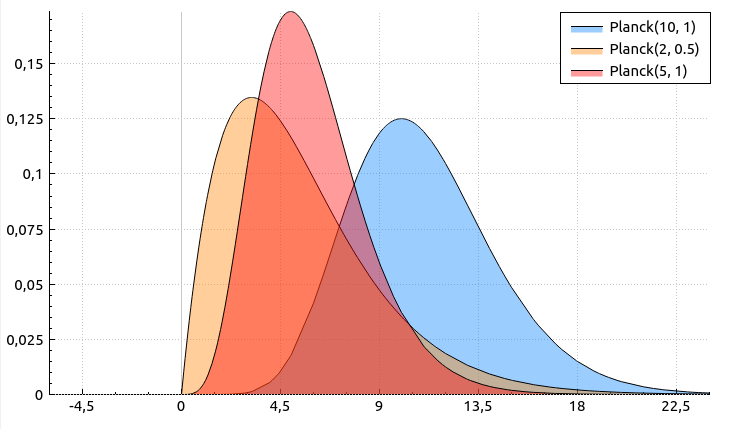
\includegraphics[width=\linewidth, right]{planck_pdf}
			\captionsetup{labelformat=empty}
			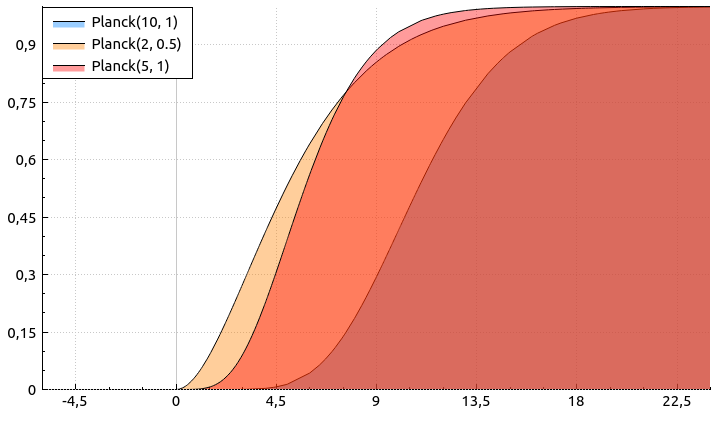
\includegraphics[width=\linewidth, right]{planck_cdf}
			\captionsetup{labelformat=empty}
		\end{minipage}
		\begin{minipage}{0.4\textwidth}
		\begin{tabular}{| r | l |}
			\hline
			Notation & $X \sim \mathrm{Planck}(a, b)$ \\
			\hline
			Parameters & $a, b > 0$ \\
			\hline
			Support & $ x \in \MR^+$  \\
			\hline
			$f(x)$ & $\frac{b^{a+1}}{\Gamma(a+1)\zeta(a+1)} \cdot \frac{x ^ a}{e^{bx} - 1}$ \\
			\hline
			$F(x)$ & Calculated numerically \\
			\hline
			$\ME[X]$ & $ \frac{(a+1)\zeta(a+2)}{b \zeta(a+1)}$ \\
			\hline
			$\Var(X)$ & $\frac{(a+1)(a+2)\zeta(a+3)}{b^2 \zeta(a+1)}  - (\ME[X])^2$ \\
			\hline
			Median & Searched numerically \\
			\hline
			Mode & $\frac{W_0(-a e^{-a}) + a}{b}$, if $a > 1$, otherwise $0$ \\
			\hline
			$\phi(t)$ & Calculated numerically \\
			\hline
		\end{tabular}
	\end{minipage}
    \end{figure}
	
	\section{Stable distribution}
	\begin{figure}[!htb]\centering
		\begin{minipage}{0.55\textwidth}
			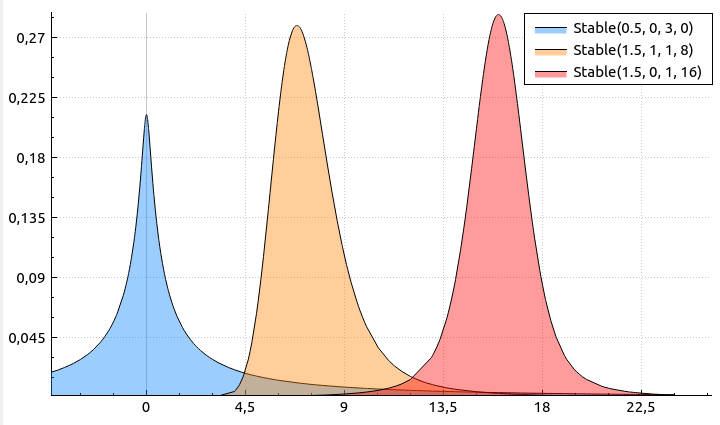
\includegraphics[width=\linewidth, right]{stable_pdf}
			\captionsetup{labelformat=empty}
			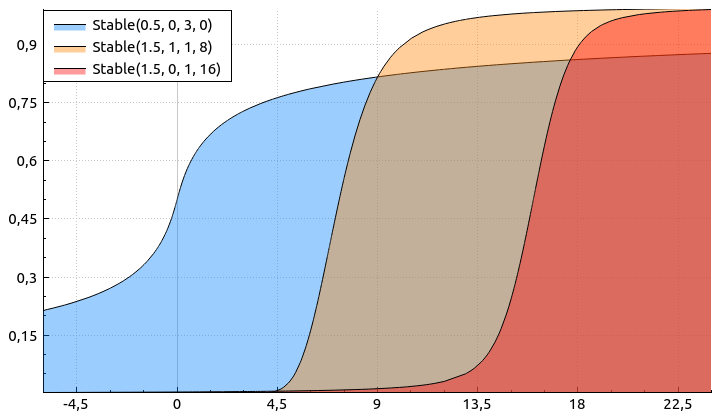
\includegraphics[width=\linewidth, right]{stable_cdf}
			\captionsetup{labelformat=empty}
		\end{minipage}
		\begin{minipage}{0.4\textwidth}
		\begin{tabular}{| r | l |}
			\hline
			Notation & $X \sim S_\alpha(\beta, \gamma, \mu)$ \\
			\hline
			Parameters & \pbox{\linewidth}{$\alpha \in (0, 2], \beta \in [-1, 1],$\\ $\gamma > 0, \mu \in \MR $} \\
			\hline
			Support & \pbox{\linewidth}{$ x \in \MR$, if  $\beta \neq 1$, \\  $ x \in [\mu, \infty)  $, if  $\beta = 1$, $\alpha < 2$, \\ $ x \in (-\infty, \mu]  $, if  $\beta = -1$, $\alpha < 2$}  \\
			\hline
			$f(x)$ & Calculated numerically \\
			\hline
			$F(x)$ & Calculated numerically \\
			\hline
			$\ME[X]$ & \pbox{\linewidth}{$ \mu$ for $\alpha > 1$,\\ otherwise undefined} \\
			\hline
			$\Var(X)$ & $2 \gamma^2 1_{\{ \alpha = 2 \} } + \infty 1_{ \{ \alpha < 2 \} }  $ \\
			\hline
			Median & \pbox{\linewidth}{$\mu$ for $\beta = 0$,\\ otherwise searched numerically} \\
			\hline
			Mode & \pbox{\linewidth}{$\mu$, if $\beta = 0$ or $\alpha = 2$, \\  $\mu + \frac{\beta \gamma}{3}$, if $|\beta| = 1$ and $\alpha = \frac{1}{2}$, \\ otherwise searched numerically} \\
			\hline
			$\phi(t)$ & $ ...$ \\
			\hline
		\end{tabular}
	    \end{minipage}
	\end{figure}
	
	\subsection{Normal distribution}
	Relation to Stable distribution:
	\[X \sim S_{2}(\cdot, \sigma^2/2, \mu) \]
	
	\begin{figure}[!htb]\centering
		\begin{minipage}{0.55\textwidth}
			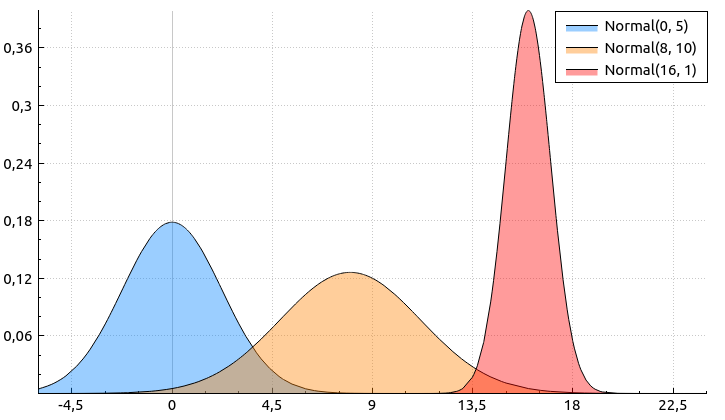
\includegraphics[width=\linewidth, right]{normal_pdf}
			\captionsetup{labelformat=empty}
			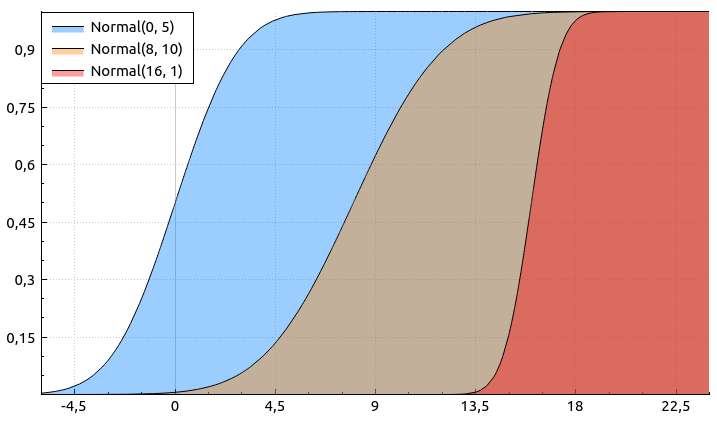
\includegraphics[width=\linewidth, right]{normal_cdf}
			\captionsetup{labelformat=empty}
		\end{minipage}
		\begin{minipage}{0.4\textwidth}
		\begin{tabular}{| r | l |}
			\hline
			Notation & $X \sim \mathcal{N}(\mu, \sigma^2)$ \\
			\hline
			Parameters & $\mu \in \MR, \sigma^2 > 0 $ \\
			\hline
			Support & $x \in \MR$  \\
			\hline
			$f(x)$ & $ \frac{1}{\sqrt{2\sigma^2\pi}}e^{-\frac{(x-\mu)^2}{2\sigma^2}}  $ \\
			\hline
			$F(x)$ & $ \frac{1}{2} \mathrm{erfc}\Big( \frac{\mu-x}{\sqrt{2\sigma^2}} \Big) $ \\
			\hline
			$\ME[X]$ & $ \mu$ \\
			\hline
			$\Var(X)$ & $\sigma^2$\\
			\hline
			Median & $\mu$ \\
			\hline
			Mode & $\mu$ \\
			\hline
			$\phi(t)$ & $ e^{i\mu t - \frac{1}{2}\sigma^2t^2}  $ \\
			\hline
		\end{tabular}
    	\end{minipage}
	\end{figure}


\subsection{Cauchy distribution}
	Relation to Stable distribution:
	\[X \sim S_{1}(0, \gamma, \mu) \]
		\begin{figure}[!htb]\centering
		\begin{minipage}{0.55\textwidth}
			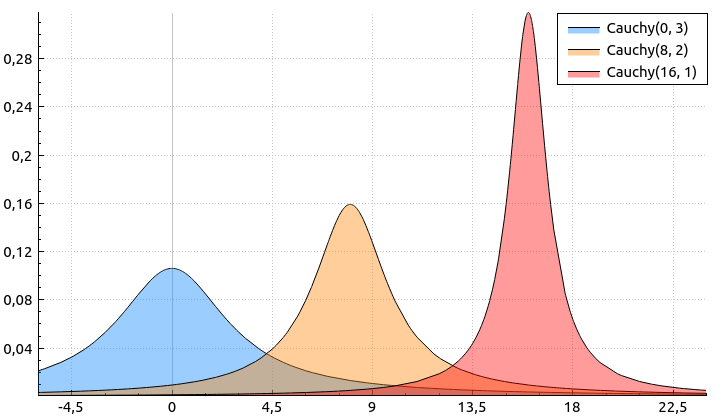
\includegraphics[width=\linewidth, right]{cauchy_pdf}
			\captionsetup{labelformat=empty}
			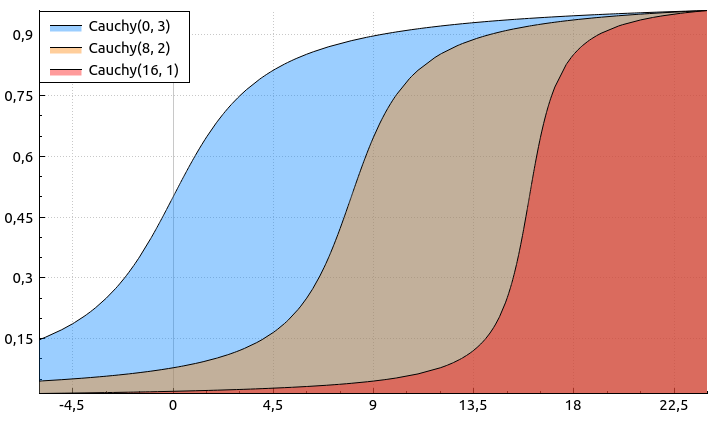
\includegraphics[width=\linewidth, right]{cauchy_cdf}
			\captionsetup{labelformat=empty}
		\end{minipage}
		\begin{minipage}{0.4\textwidth}
		\begin{tabular}{| r | l |}
			\hline
			Notation & $X \sim \mathrm{Cauchy}(\mu, \gamma)$ \\
			\hline
			Parameters & $\mu \in \MR, \gamma^2 > 0 $ \\
			\hline
			Support & $x \in \MR$  \\
			\hline
			$f(x)$ & $ \frac{1}{ \pi \gamma \Big[ 1 + \big( \frac{x-\mu}{\gamma} \big)^2 \Big]  }  $ \\
			\hline
			$F(x)$ & $ \frac{1}{\pi} \mathrm{atan}\Big( \frac{x-\mu}{\gamma} \Big) + \frac{1}{2} $ \\
			\hline
			$\ME[X]$ & Undefined \\
			\hline
			$\Var(X)$ & $\infty $\\
			\hline
			Median & $\mu$ \\
			\hline
			Mode & $\mu$ \\
			\hline
			$\phi(t)$ & $ e^{i\mu t - \gamma |t|}  $ \\
			\hline
		\end{tabular}
	    \end{minipage}
	\end{figure}
	
	
\subsection{Levy distribution}
	Relation to Stable distribution:
	\[X \sim S_{\frac{1}{2}}(1, \gamma, \mu) \]


\subsection{Holtsmark distribution}
	Relation to Stable distribution:
	\[X \sim S_{\frac{3}{2}}(0, \gamma, \mu) \]


\subsection{Landau distribution}
	Relation to Stable distribution:
	\[X \sim S_{1}(1, \gamma, \mu) \]
	
	
\section{Pareto distribution}
			\begin{figure}[!htb]\centering
				\begin{minipage}{0.55\textwidth}
					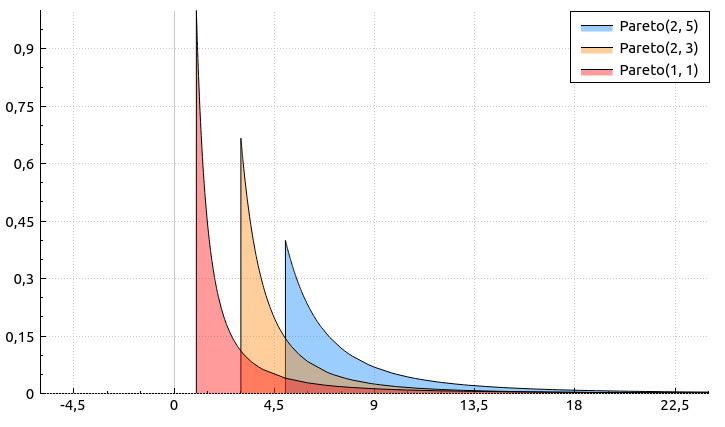
\includegraphics[width=\linewidth, right]{pareto_pdf}
					\captionsetup{labelformat=empty}
					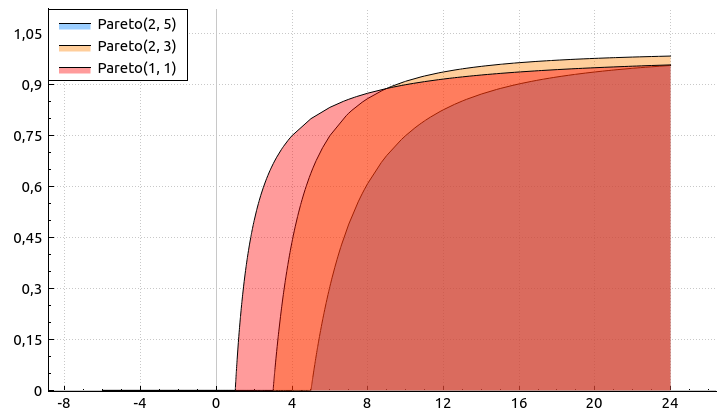
\includegraphics[width=\linewidth, right]{pareto_cdf}
					\captionsetup{labelformat=empty}
				\end{minipage}
				\begin{minipage}{0.4\textwidth}
					\begin{tabular}{| r | l |}
						\hline
						Notation & $X \sim \mathrm{Pareto}(\alpha, \sigma)$ \\
						\hline
						Parameters & $\alpha,  \sigma > 0 $ \\
						\hline
						Support & $x \geq \sigma$  \\
						\hline
						$f(x)$ & $ \frac{\alpha \sigma^\alpha}{x^{\alpha+1}}  $ \\
						\hline
						$F(x)$ & $ 1-\big( \frac{\sigma}{x} \big)^\alpha $ \\
						\hline
						$\ME[X]$ & \pbox{\linewidth}{$ \frac{\alpha\sigma}{\alpha-1}$ for $\alpha > 1$, \\ $\infty$ otherwise} \\
						\hline
						$\Var(X)$ & \pbox{\linewidth}{$\frac{\sigma^2 \alpha}{(\alpha-1)^2(\alpha-2)}$ for $\alpha > 2$, \\ $\infty$ otherwise } \\
						\hline
						Median & $\sigma 2^{1/\alpha}$ \\
						\hline
						Mode & $\sigma$ \\
						\hline
						$\phi(t)$ & Calculated numerically \\
						\hline
					\end{tabular}
				\end{minipage}
			\end{figure}
    
	\paragraph{Estimation of parameters.}
	\subparagraph{Frequentist inference.} Log-likelihood function is
	\[
	\ln \mathcal{L}(\alpha, \sigma | X) = n \ln \alpha + n \alpha \ln \sigma - (\alpha + 1) \sum_{i=1}^{n} \ln X_i.
	\]
	We assume that $\sigma \leq X_{(1)}$, otherwise sample $X$ couldn't have been generated from such distribution. It is obvious, that $\ln \mathcal{L}(\alpha, \sigma | X)$ is an increasing function in terms of $\sigma$, therefore $\hat{\sigma} = X_{(1)}$ is an optimal estimator.
	Let's take derivative with respect to $\alpha$:
	\[
	\frac{\partial \ln \mathcal{L}(\alpha, \sigma | X) }{\partial \alpha} = \frac{n}{\alpha} + n \ln \sigma - \sum_{i=1}^{n} \ln X_i.
	\]
	From this we conclude that the maximum-likelihood estimator of shape is
	\[
	\hat{\alpha} = \frac{1}{ \frac{1}{n} (\sum_{i=1}^{n} \ln X_i) - \ln \hat{\sigma} }.
	\]
	It is known that $\hat{\sigma} \sim \mathrm{Pareto}(n\alpha, \sigma)$ and $\hat{\alpha} \sim \operatorname{Inv-\Gamma}(n-1, n\alpha)$ and they are independent. Then
	\[ \ME[\hat{\sigma}] = \frac{ \sigma}{1-\frac{1}{n \alpha}}\]
	and
	\[ \ME[\hat{\alpha}] = \frac{n\alpha}{n-2}. \]
	Therefore, in order to get unbiased estimators we need to make the following transformations:
	\[ \tilde{\alpha} = \frac{n-2}{n}\hat{\alpha} \quad \text{and} \quad \tilde{\sigma} = \hat{\sigma} \bigg(1 - \frac{1}{(n-1)\hat{\alpha}}\bigg). \]
	Note that if we estimate parameters separately, then $\hat{\alpha} \sim \operatorname{Inv-\Gamma}(n, n\alpha)$ and transformations are different.
	
	\subparagraph{Bayesian inference.} We now assume that $\sigma$ is known and prior distribution of $\alpha$ is $\Gamma(\kappa, \beta)$:
	\[
	h(\alpha) = \frac{\beta^\kappa}{\Gamma(\kappa)} \alpha^{\kappa-1}e^{-\beta \alpha}.
	\]
	The density of posterior distribution is
	\[
	f(\alpha | X) \propto \prod_{i=1}^n \frac{\sigma^\alpha}{{X_i}^{\alpha-1}} \cdot \alpha^{\kappa+n-1}e^{-\beta \alpha} \propto \alpha^{\kappa+n-1} e^{ -(\beta + \sum_{i=1}^n \ln (X_i/\sigma))\alpha }.
	\]
	Therefore, $\alpha |X \sim \Gamma(\kappa + n, \beta +\sum_{i=1}^n \ln (X_i/\sigma))$ and Bayesian estimator is
	\[ \ME[\alpha | X] = \frac{\kappa + n}{ \beta +\sum_{i=1}^n \ln (X_i/\sigma) }. \]
	MAP estimator is
	\[ \alpha_{MAP} = \frac{\kappa + n-1}{ \beta +\sum_{i=1}^n \ln (X_i/\sigma) }. \]
	\textit{Note on fitting scale with Bayes:} let it be vice versa, $\alpha$ is known while $\sigma$ is not. Then we say that a priori $\sigma \sim \operatorname{Pareto}(\kappa, \theta)$:
	\[
	h(\sigma) = \frac{\kappa\theta^\kappa}{\sigma^{\kappa+1}}.
	\]
	Then posterior distribution is:
	\[
	f(\sigma|X) \propto \prod_{i=1}^n \frac{1}{{X_i}^{\alpha-1}} \cdot \sigma^{\alpha n - \kappa - 1} \mathbf{1}_{ \{ \theta < \sigma < X_{(1)}\} } \sim \operatorname{Bounded-Pareto}(\kappa-\alpha n, \theta, X_{(1)}).
	\]
	This imposes the following additional constraints on the prior hyperparameters: $\kappa > \alpha n$ and $\theta < X_{(1)}$. Bayesian estimator:
	\[
	\ME[\sigma|X] = \frac{\theta^{\alpha'}}{1-\Big(\frac{\theta}{X_{(1)}}\Big)^{\alpha'}} \cdot \Big(\frac{\alpha'}{\alpha'-1}\Big)\cdot \bigg( \frac{1}{\theta^{\alpha'}} -\frac{1}{X_{(1)}^{\alpha'}} \bigg)
	\]
	with $\alpha'=\kappa - \alpha n$.
	MAP estimator is just
	\[
	\sigma_{MAP} = \theta.
	\]
	However, Bounded-Pareto distribution is not yet supported.
	
\section{Weibull}

\begin{figure}[!htb]\centering
	\begin{minipage}{0.55\textwidth}
		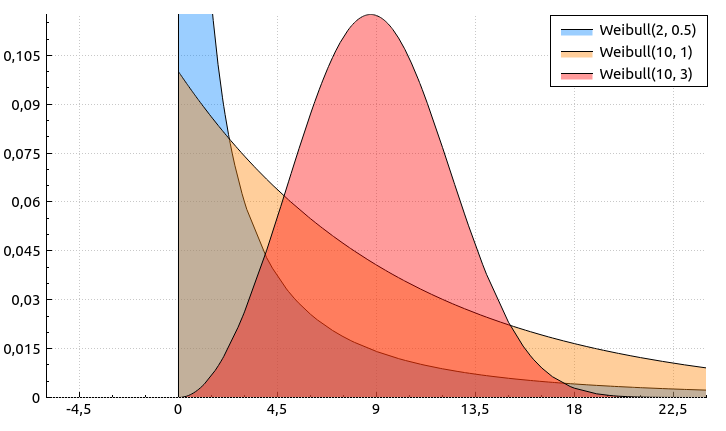
\includegraphics[width=\linewidth, right]{weibull_pdf}
		\captionsetup{labelformat=empty}
		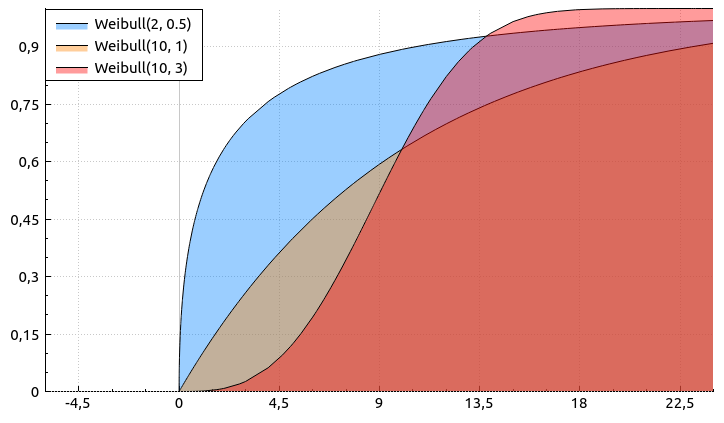
\includegraphics[width=\linewidth, right]{weibull_cdf}
		\captionsetup{labelformat=empty}
	\end{minipage}
	\begin{minipage}{0.4\textwidth}
		\begin{tabular}{| r | l |}
			\hline
			Notation & $X \sim \mathrm{Weibull}(\lambda, k)$ \\
			\hline
			Parameters & $\lambda, k > 0 $ \\
			\hline
			Support & $x \in \MR^+$  \\
			\hline
			$f(x)$ & $ \frac{k}{\lambda}\big( \frac{x}{\lambda}\big)^{k-1} \exp(-(x/\lambda)^k)  $ \\
			\hline
			$F(x)$ & $ 1-\exp(-(x/\lambda)^k) $ \\
			\hline
			$\ME[X]$ & $ \lambda \Gamma(1+1/k)$ \\
			\hline
			$\Var(X)$ & $\lambda^2 \Gamma(1+2/k) - (\ME[X])^2$ \\
			\hline
			Median & $\lambda (\ln2)^{\frac{1}{k}}$ \\
			\hline
			Mode & $\lambda \big( 1-\frac{1}{k} \big)^{\frac{1}{k}}$ \\
			\hline
			$\phi(t)$ & Calculated numerically \\
			\hline
		\end{tabular}
	\end{minipage}
\end{figure}
\paragraph{Estimation of scale}.
\subparagraph{Frequentist inference.} Log-likelihood function:
\[
\ln \mathcal{L}(\lambda, k|X) = n (\ln k - \ln \lambda) + (k-1)\sum_{i=1}^{n}(\ln X_i - \ln \lambda) - \frac{1}{\lambda^k}\sum_{i=1}^{n} X_i^k.
\]
The derivative with respect to scale:
\[
\frac{\partial\ln \mathcal{L}(\lambda, k|X) }{\partial \lambda} = -\frac{n k}{\lambda} + \frac{k}{\lambda^{k+1}} \sum_{i=1}^{n} X_i^k=0.
\]
Therefore, maximum-likelihood estimation for $\lambda$ is
\[
\hat{\lambda} = \bigg(\sum_{i=1}^{n}X_i^k\bigg)^{\frac{1}{k}}.
\]
\subparagraph{Bayesian inference.} Assume $k$ is known. Instead of estimating $\lambda$ we give an estimation for $\lambda^k$. Let's say that prior distribution of $\lambda^k$ is $\operatorname{Inv-\Gamma}(\alpha, \beta)$:
\[
h(\lambda^k) = \frac{\beta^\alpha}{\Gamma(\alpha)} \lambda^{-k(\alpha+1)} e^{-\beta / \lambda^k}.
\]
Posterior distribution then:
\[
f(\lambda^k| X) \propto \lambda^{-k(\alpha+1+n)} e^{-\frac{1}{\lambda^k} (\beta+\sum_{i=1}^{n}X_i^k)} \sim \operatorname{Inv-\Gamma}(\alpha+n, \beta+\sum_{i=1}^{n}X_i^k).
\]
Bayesian estimator:
\[
\ME[\lambda^k|X] = \frac{\beta+\sum_{i=1}^{n}X_i^k}{\alpha+n-1},
\]
MAP estimator:
\[
\lambda_{MAP}^k = \frac{\beta+\sum_{i=1}^{n}X_i^k}{\alpha+n+1}.
\]

	\pagebreak
	\part{Discrete univariate distributions}
	\section{Beta-binomial distribution}
	\section{Binomial distribution}
	\begin{center}
		\begin{tabular}{| r | l |}
			\hline
			Notation & $ X \sim \mathrm{Bin}(n, p) $ \\
			\hline
			Parameters & $ n \in \MN, p \in [0, 1]  $ \\
			\hline
			Support & $ k \in \{0, \dots, n  \} $  \\
			\hline
			P.m.f. & $\MP(X = k) = \binom{n}{k} p^k (1-p)^{n-k}  $ \\
			\hline
			$F(x)$ & $\MP(X \leq k)=I_{1-p}(n-k, 1+k) $ \\
			\hline
			$\ME[X]$ & $ np$ \\
			\hline
			$\Var(X)$ & $np(1-p)$ \\
			\hline
			Median & $[np]$ \\
			\hline
			Mode & $[(n+1)p]$ \\
			\hline
			$\phi(t)$ & $ (1-p+pe^{it})^n  $ \\
			\hline
		\end{tabular}
	\end{center}
	\subsection{Bernoulli}
	Notation:
	\[ X \sim \mathrm{Bernoulli}(p). \]
	Relation to Binomial distribution: \[X \sim \mathrm{Bin}(1, p). \]
	\section{Poisson distribution}
	\begin{center}
		\begin{tabular}{| r | l |}
			\hline
			Notation & $ X \sim \mathrm{Po}(\lambda) $ \\
			\hline
			Parameters & $\lambda > 0$ \\
			\hline
			Support & $ k \in \MN_0 $  \\
			\hline
			P.m.f. & $\MP(X = k) = \frac{\lambda^k e^{-\lambda}}{k!}$ \\
			\hline
			$F(x)$ & $\MP(X \leq k)=Q(k+1, \lambda)$ \\
			\hline
			$\ME[X]$ & $ \lambda$ \\
			\hline
			$\Var(X)$ & $\lambda$ \\
			\hline
			Median & $\sim \max\big([\lambda + \frac{1}{3} - \frac{0.02}{\lambda}], 0\big) $ \\
			\hline
			Mode & $[\lambda]$ \\
			\hline
			$\phi(t)$ & $ \exp \{ \lambda(e^{it}-1) \}  $ \\
			\hline
		\end{tabular}
	\end{center}
	
	Generator (let $\delta = \mu \in \mathbb{Z}$). (There is a mistake in Lemma 3.8 in first inequality). Recall that
	\[ q(X) = X \ln(\lambda) - \ln \Big( \frac{(\mu + X)!}{\mu!} \Big). \]
	
	We denote acceptance probability $\MP(W \leq q(X))$ by $p$.
	\begin{itemize}
		
		\item $k = \mu$. Probability to be in this setting is $1 / c$.
		\[\MP(X = 0 | W \leq q(X)) = \frac{\MP(X = 0, W \leq q(X))}{\MP(W \leq q(X))} = \frac{1}{pc}. \]
		On the other hand it should be equal to:
		\[ \frac{1}{pc} = \frac{\lambda^\mu e^{-\lambda}}{\mu!}. \]
		\item $k = \mu + 1$.
		\[
		\begin{aligned}
		\MP(X = 1 | W \leq q(X)) &= \frac{\MP(X = 1, W \leq q(X))}{\MP(W \leq q(X))} = \frac{\lambda}{p(\mu + 1) c} \\
		&= \frac{\lambda^{\mu+1} e^{-\lambda}}{(\mu + 1)!}.
		\end{aligned}
	    \]
		
		
		\item $k < \mu$. Here was mistake in the book. We adjust the probabilities. Probability to be in this setting is $\sqrt{\pi \mu / 2 e} / c$.
		\[
		\begin{aligned}
		\MP(W \leq q(X), X = k - \mu | U \leq c_1) &= \MP\Bigg(-\frac{N^2}{2} + \frac{1}{2} - E < q( \lfloor -|N|\sqrt{\mu} \rfloor ), \lceil |N| \sqrt{\mu} \rceil = \mu-k \Bigg) \\
		& = \MP\Bigg(-\frac{N^2}{2} + \frac{1}{2} - E < \lfloor -|N|\sqrt{\mu} \rfloor \ln(\lambda) - \ln\bigg( \frac{(\mu + \lfloor -|N|\sqrt{\mu} \rfloor)!}{\mu!} \bigg), 
		\\& \qquad\qquad \frac{\mu-k-1}{\sqrt{\mu}} \leq |N| < \frac{\mu-k}{\sqrt{\mu}} \Bigg)	\\
		& = \MP\Bigg(U < \exp \Big \{\frac{N^2}{2}  - \frac{1}{2} + \lfloor -|N|\sqrt{\mu} \rfloor \ln(\lambda) - \ln\bigg( \frac{(\mu + \lfloor -|N|\sqrt{\mu} \rfloor)!}{\mu!} \bigg) \Big\}, 
		\\& \qquad\qquad \frac{\mu-k-1}{\sqrt{\mu}} \leq |N| < \frac{\mu-k}{\sqrt{\mu}}   \Bigg) \\
		&= \sqrt{\frac{2}{e\pi}} \int_{\frac{\mu-k-1}{\sqrt{\mu}}}^{\frac{\mu-k}{\sqrt{\mu}}}  \exp \Big \{ \lfloor -|n|\sqrt{\mu} \rfloor \ln(\lambda) - \ln\bigg( \frac{(\mu + \lfloor -|n|\sqrt{\mu} \rfloor)!}{\mu!} \bigg) \Big\} dn \\
		& = \sqrt{\frac{2}{e\pi \mu}} \int_{\mu-k-1}^{\mu-k}  \exp \Big \{ \lfloor -z \rfloor \ln(\lambda) - \ln\bigg( \frac{(\mu + \lfloor -z \rfloor)!}{\mu!} \bigg) \Big\} dz \\
		& = \sqrt{\frac{2}{e\pi \mu}} \exp \Big \{ (k-\mu) \ln(\lambda) - \ln\bigg( \frac{k!}{\mu!} \bigg) \Big\} \\
		& = \sqrt{\frac{2}{e\pi \mu}} \lambda^{k-\mu} \frac{\mu!}{k!}
		\end{aligned} 
		\]
		
		Hence,
		\[ 
		\begin{aligned}
		\MP(X = k - \mu | W \leq q(X)) &= \frac{\MP(W \leq q(X), X = k - \mu) }{\MP(W \leq q(X))} \\
		&= \sqrt{\frac{2}{\pi \mu e}} \lambda^{k-\mu} \frac{\mu!}{k!} \cdot \sqrt{\pi \mu e / 2} \frac{\lambda^\mu e^{-\lambda}}{\mu!} \\
		&= \frac{\lambda^{k} e^{-\lambda}}{k!}
		\end{aligned} 
		\]
		
		\item $k \in [\mu + 2, 2 \mu]$. Probability to be in this setting is $\sqrt{\frac{3\pi \mu}{4}} e^{\frac{1}{3\mu}} / c$. We also have
		\[ W = \frac{-Y^2+2Y}{3\mu} - E = \frac{1}{3\mu}-\frac{N^2}{2} - E. \]
		Then
		\[
		\begin{aligned}
		\MP(W \leq q(X) | X = k-\mu | U \in ...) &= \MP\Bigg(\frac{1}{3\mu}-\frac{N^2}{2} - E < q( \lceil 1+|N| \sqrt{3\mu/2} \rceil ),
		\lceil 1+|N| \sqrt{3\mu/2} \rceil = k - \mu\Bigg) \\
		& = \MP\Bigg(U < \exp \Big \{-\frac{1}{3\mu} + \frac{N^2}{2} + q( \lceil 1+|N| \sqrt{3\mu/2} \rceil ) \Big\}, \\ 
		& \qquad \qquad \frac{k-\mu-2}{\sqrt{3\mu/2}} < |N| \leq \frac{k-\mu-1}{\sqrt{3\mu/2}} \Bigg) \\
		& = \sqrt{\frac{2}{\pi}} e^{-\frac{1}{3\mu}} \int_{\frac{k-\mu-2}{\sqrt{3\mu/2}}}^{\frac{k-\mu-1}{\sqrt{3\mu/2}}} \exp \Big \{  q( \lceil 1+|n| \sqrt{3\mu/2} \rceil ) \Big\} dn \\
		& =  \sqrt{\frac{4}{3\pi\mu}} e^{-\frac{1}{3\mu}}  \int_{k-\mu-1}^{k-\mu} \exp \Big \{ \lceil z \rceil \ln(\lambda) - \ln\bigg( \frac{(\mu + \lceil z \rceil)!}{\mu!} \bigg) \Big\} dz \\
		& = \sqrt{\frac{4}{3\pi\mu}} e^{-\frac{1}{3\mu}}\mu! \frac{\lambda^{k-\mu}}{k!}.
		\end{aligned}
		\]
		
		
		\item $k > 2\mu$. Probability to be in this setting is $6e^{-\frac{2+\mu}{6}} / c$.
		\[
		\begin{aligned}
		\MP(W \leq q(X) | X = k - \mu | U \in ...) &= \MP\Big(-\frac{2 + \mu}{6} - V - E < q( \lceil \mu + 6V \rceil ), \lceil \mu + 6V \rceil = k - \mu \Big)  \\
		& = \MP\Bigg(-\frac{2 + \mu}{6} - V + \ln(U) < \lceil \mu + 6V \rceil \ln(\lambda) - \ln \bigg( \frac{(\mu + \lceil \lambda + 6V \rceil)!}{\mu!} \bigg),\\
		& \qquad \qquad \lceil \mu + 6V \rceil = k - \mu \Bigg) \\
		& =	\MP \Bigg( U < \exp\bigg\{\frac{2 + \mu}{6} + V + \lceil \mu + 6V \rceil \ln(\lambda) - \ln \bigg( \frac{(\mu + \lceil \mu + 6V \rceil)!}{\mu!} \bigg) \bigg\},\\
		& \qquad \qquad \frac{k - 2\mu - 1}{6} < V \leq \frac{k - 2\mu}{6} \Bigg) \\
		& = \int_{\frac{k - 2\mu - 1}{6}}^{\frac{k - 2\mu}{6}} \exp\bigg\{\frac{2 + \mu}{6} + \lceil \mu + 6v \rceil \ln(\lambda) - \ln \bigg( \frac{(\mu + \lceil \mu + 6v \rceil)!}{\mu!} \bigg) \bigg\} dv \\
		& = \frac{ e^{\frac{2+\lambda}{6}}}{6} \int_{k-\mu-1}^{k-\mu} \exp\bigg\{\lceil z \rceil \ln(\lambda) - \ln \bigg( \frac{(\mu + \lceil z \rceil)!}{\mu!} \bigg) \bigg\} dz \\
		& = \frac{ e^{\frac{2+\lambda}{6}}}{6} \exp\bigg\{(k-\mu) \ln(\lambda) - \ln \bigg( \frac{k!}{\mu!} \bigg) \bigg\} \\
		& = \frac{ e^{\frac{2+\lambda}{6}}}{6} \lambda^{k-\mu} \frac{\mu!}{k!}
		\end{aligned} 
		\]
		Hence,
		\[ 
		\begin{aligned}
		\MP(X = k - \mu | W \leq q(X)) &= \frac{\MP(W \leq q(X), X = k-\mu)}{\MP(W \leq q(X))} \\
		& = \frac{ e^{\frac{2+\lambda}{6}}}{6} \lambda^{k-\mu} \frac{\mu!}{k!} \cdot \frac{6e^{-\frac{2+\mu}{6}}}{pc}\\
		& = \frac{\lambda^k e^{-\lambda}}{k!}
		\end{aligned} 
		\]
		
	\end{itemize}
	\pagebreak
	\part{Bivariate distributions}
	\section{Bivariate Normal distribution}
	\section{Normal-Inverse-Gamma distribution}
	\section{Trinomial distribution}
	
	\pagebreak
	\part{Circular distributions}
	\section{von Mises distribution}
	\section{Wrapped Exponential distribution}
	
	\pagebreak
	\part{Singular distributions}
	\section{Cantor distribution}
	
\end{document}
